\section{Utilisation}
\label{section:utilisation}
	\subsection{Menu Principal}
		Lorsque le joueur lance le jeu, il se retrouve face au menu principal (Figure \ref{fig:main_menu}). Plusieurs choix s'offrent à lui:
		\begin{itemize}
			\item Lancer une nouvelle partie
			\item Charger une partie enregistrée ; malheureusement, cette fonctionnalité n'a pas pu être complétée dans les temps impartis, et a donc du être retirée de cette version !
			\item Quitter le jeu
		\end{itemize}

		\begin{figure}[h]
			\centering
			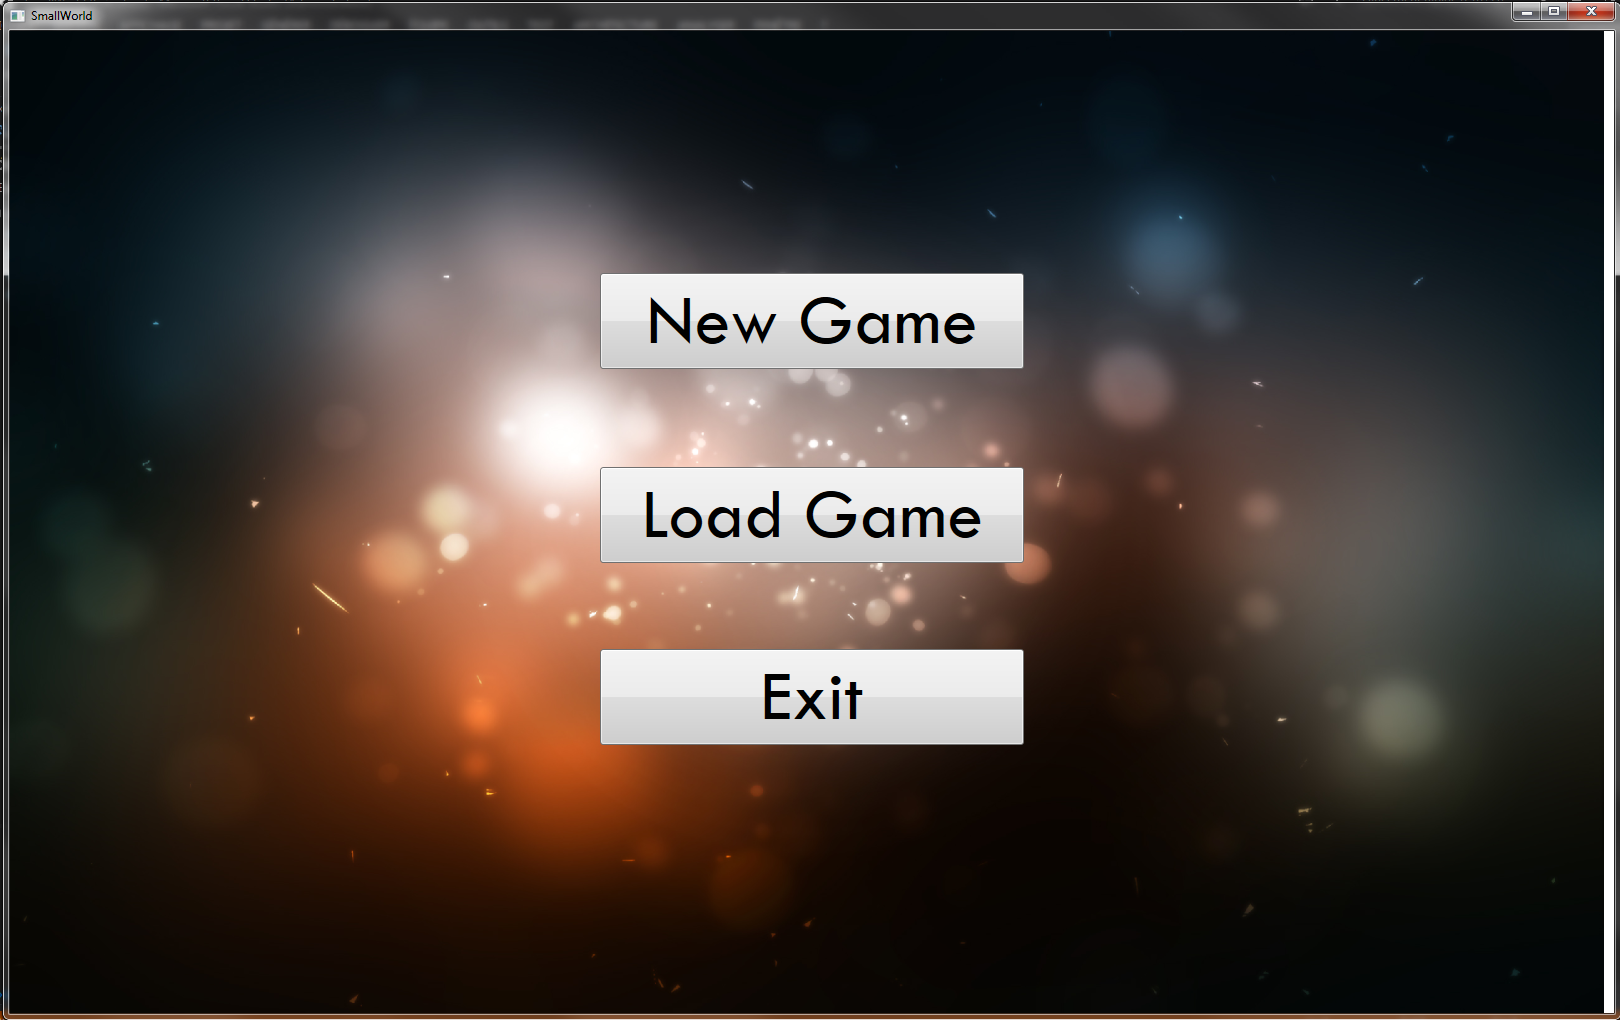
\includegraphics[width=1\textwidth]{figure/main_menu.png}
			\caption{L'interface spartiate du menu principal permet à l'utilisateur de se concentrer sur ses choix existentiels.}
			\label{fig:main_menu}
		\end{figure}


	\subsection{Nouvelle partie}
		Si l'utilisateur choisit de lancer une nouvelle partie, il se retrouvera face à l'interface de création de partie (Figure \ref{fig:new_game}). Il pourra régler les noms de joueurs, ainsi que leurs factions, et la taille de la carte souhaitée. A noter que le jeu ne se lancera pas si les deux joueurs possèdent la même faction. Enfin, la taille de la carte choisie fera aussi varier le nombre d'unités de chaque joueurs.

		\begin{figure}[h]
			\centering
			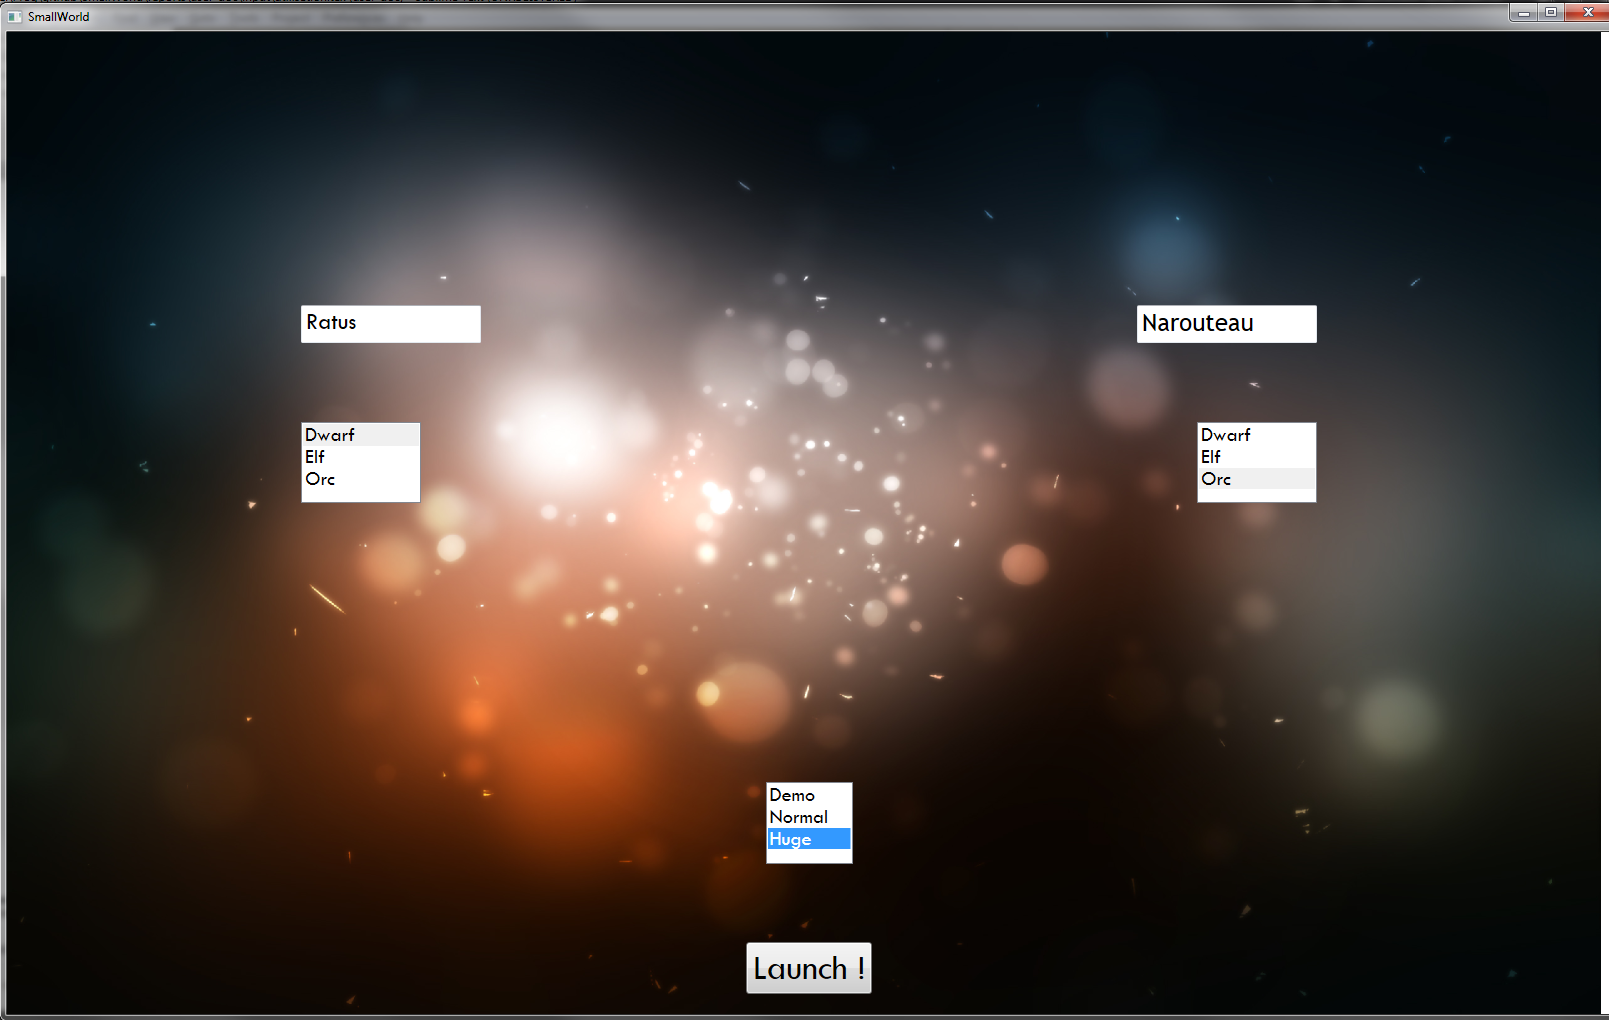
\includegraphics[width=1\textwidth]{figure/new_game.png}
			\caption{Un total de 5 options permettent de ne jamais rejouer deux fois la même partie.}
			\label{fig:new_game}
		\end{figure}

		Lorsqu'il est satisfait de ses réglages, il peut cliquer sur \og Launch ! \fg, et ainsi lancer la partie.

	\subsection{Interface de jeu}
		L'interface de jeu (Figure \ref{fig:in_game}) se décompose en deux grandes zones:
		\begin{itemize}
			\item Les informations des joueurs (en haut)
			\item Le plateau de jeu
		\end{itemize}

		\begin{figure}[h]
			\centering
			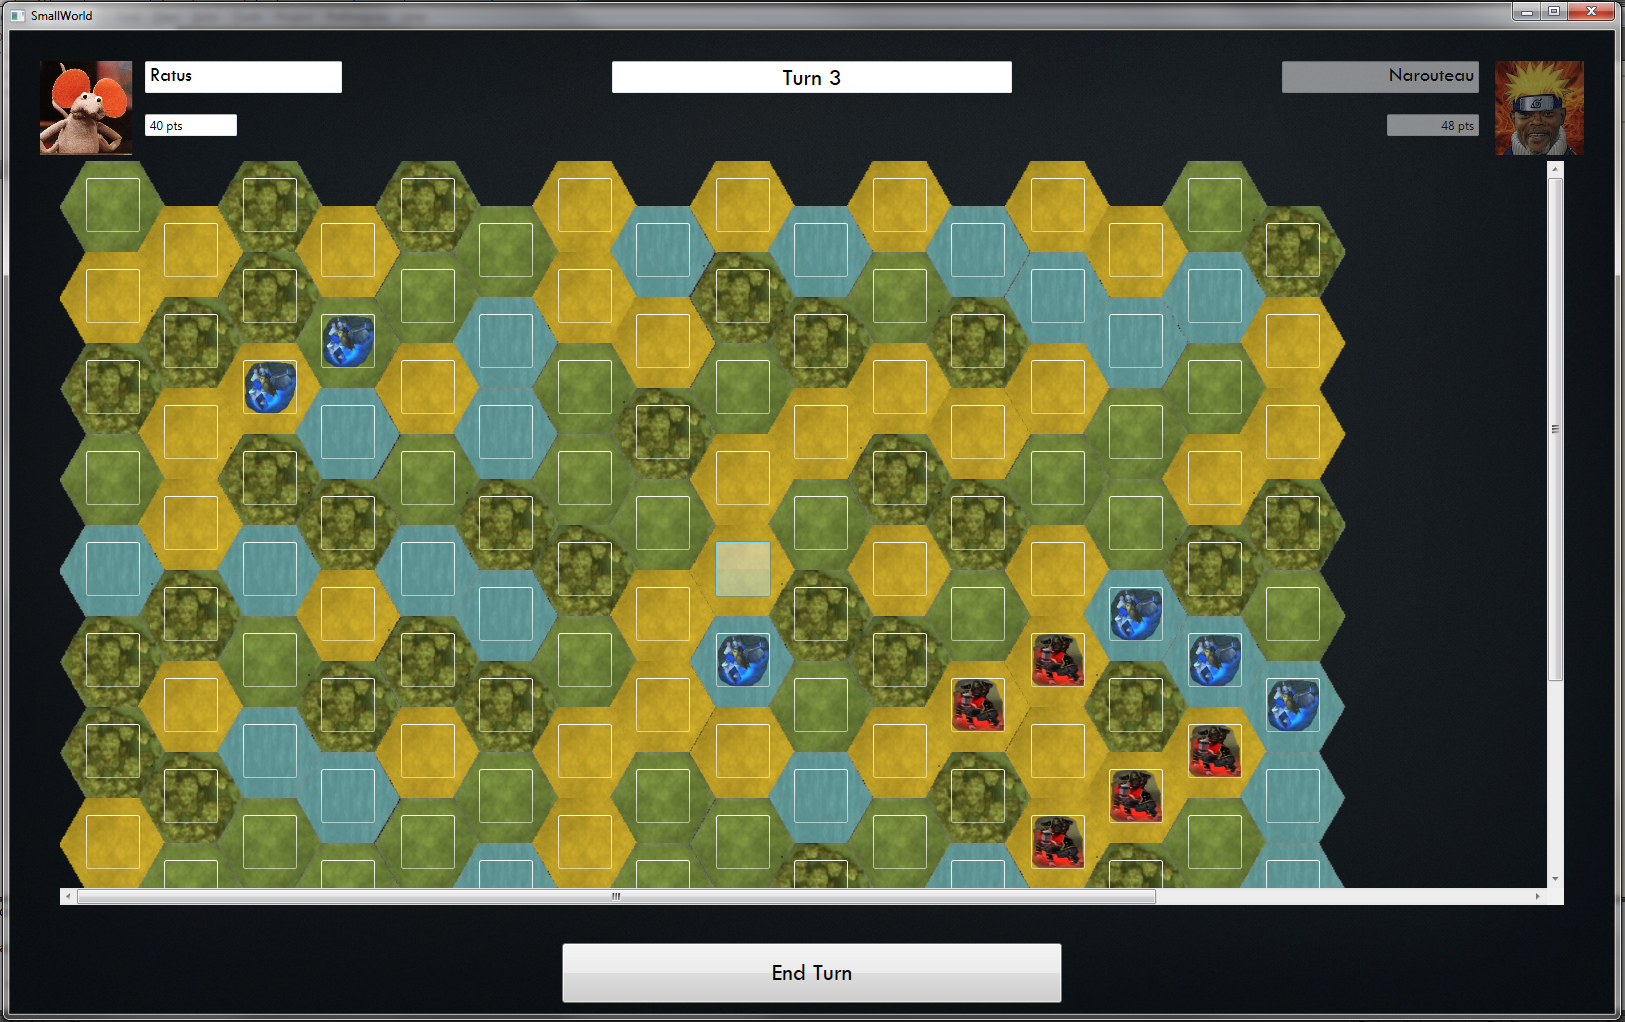
\includegraphics[width=1\textwidth]{figure/in_game.png}
			\caption{Les différentes informations utiles sont facilement lisibles.}
			\label{fig:in_game}
		\end{figure}

		Les informations du joueur actif ont une opacité supérieure à celle du joueur en attente (dans notre exemple, c'est au tour de Ratus de jouer).

		Pour sélectionner une unité, il suffit de cliquer dessus. Un clic sur la case de destination déplacera l'unité si elle remplit les conditions requise. Il en va de même pour les combats, où sélectionner son unité puis cliquer sur la cible sert à déclencher une bataille sanglante et sans mercis.

		Une fois qu'un joueur aura fini son tour, il lui suffira de cliquer sur le bouton \og End Turn \fg, intelligemment placé en bas de l'écran.

		Lorsque la partie sera terminée, le jeu passera automatiquement à l'écran de victoire.

	\subsection{Ecran de victoire}
		Afin de ne pas gâcher la surprise, l'écran de victoire ne sera pas représenté dans ce guide. Le lecteur est donc invité à jouer au jeu pour pouvoir contempler cette œuvre d'art : )

		A noter que dans la version actuelle du jeu, il faut relancer l’exécutable si on veut lancer une nouvelle partie. Une lacune qui saura être corrigée dans les prochaines version...